%% LatentSky — AGU Advances manuscript
%% Compile on Overleaf with the official AGU template (class agujournal2019),
%% or drop agujournal2019.cls + agutexSI2019.cls into this folder.
%% Structure follows the group-meeting deck (deck/build.py): model and flow matching first,
%% then the rain decomposition (skill by scale), then the horizon; WB2 is the outlook.

\documentclass[draft]{agujournal2019}
\usepackage{url}
\usepackage{lineno}
\usepackage[inline]{trackchanges}
\usepackage{soul}
\linenumbers

\journalname{AGU Advances}

\begin{document}

\title{The Size of the Storm Sets the Horizon: a Scale-Aware Evaluation of
AI Precipitation Forecasts}
%% alt candidates:
%%  - A Scale-Aware Predictability Horizon for AI Precipitation Forecasts
%%  - How Far Ahead Can AI Predict Rain? A Scale-Aware Predictability Horizon

\authors{Sophie Abramian\affil{1}, Tim Zhou\affil{2}, Sara Shamekh\affil{2}}
\affiliation{1}{Columbia University, New York, NY, USA}
\affiliation{2}{New York University, New York, NY, USA}
\correspondingauthor{Sophie Abramian}{sophieabramian@gmail.com}

%% ===================== KEY POINTS (three, <= 140 chars each) ================
\begin{keypoints}
\item Flow matching turns a blurred deterministic rain forecast into sharp
draws that carry the intensities and the small scales of the truth
\item Split into systems of intensity times area, the flow detects more at
every size and removes the too-large, too-weak bias, at a false-alarm cost
\item The detection horizon grows with system size as a power law of exponent
1.6; operational AI forecasts show the same size-dependent limits
\end{keypoints}

%% ===================== ABSTRACT ============================================
\begin{abstract}
%% DRAFT for Sophie's rewrite
How far ahead precipitation can be predicted depends on the size of the
precipitating system, yet the pixel-wise scores by which AI forecasts are
usually ranked integrate over scale, and mean-square-error training blurs
the small systems the question is about. Using a 40-day kilometer-scale DYAMOND MPAS integration,
we first build a forecast that is realistic at every scale. A deterministic
U-Net trained on mean-square error returns the conditional mean --- the right
pattern, blurred. A conditional rectified flow, trained to transport that
forecast to the truth along its own measured error, returns sharp draws. We
then ask how skill is distributed across scales: every precipitating system
is decomposed into an area and an intensity ($P = \rho A$) and matched
between forecast and truth. At $+3$~h detection rises from $0.04$ for
$30$-km systems to $0.98$ at $480$~km; the flow detects more than the U-Net
in every size band, removes its too-large, too-weak bias per draw, and pays
an explicitly priced false-alarm cost below $65$~km. Finally we define a
scale-dependent detection horizon $T(L)$ --- the e-folding time of the
probability of detection per size band --- with persistence as a nested
null. Conditional on a perfectly known large-scale state, the horizon follows
a power law $T(L) \propto L^{\alpha}$ with $\alpha = 1.63$ for the flow,
$1.79$ for the U-Net, and $1.41$ for persistence: a $30$-km convective cell
is lost within the hour, a $500$-km system survives beyond a day, and below
${\sim}100$~km only the flow keeps up with persistence. Applied unchanged to
operational AI models (GraphCast, FuXi, GenCast, FGN), the same
scale-dependent limits hold: sampling a diffusion member restores intensity
from $150$~km up, while below $60$~km no model detects systems --- a limit
set jointly by $0.25^{\circ}$ resolution and by forecast steps far beyond the
small-system horizon.
\end{abstract}

\section*{Plain Language Summary}
%% DRAFT for Sophie's rewrite
How far ahead can rain be predicted? It depends on the rain: a monsoon rain
shield hundreds of kilometers wide will still be there tomorrow, but a small
thunderstorm may not survive the next hour. To measure this, a forecast must
first draw small storms at all, and most do not. Models trained to minimize
the average error respond to uncertainty by blurring --- they draw storms too
large and too weak. We train a second network that learns to turn the blurred
forecast into sharp, realistic possibilities, the way one photo can be
brought into several plausible focuses. We then treat every rainy patch in a
very high resolution simulation as an object with a size and an intensity,
and count how many objects of each size a forecast finds. The sharp forecast
finds more storms of every size and draws them with the right size and
strength --- at the price of more false alarms among the smallest, which we
report. Following these counts as the forecast reaches further ahead gives a
simple law: the survival time of predictions grows steeply with storm size.
Today's operational AI weather models show the same behavior: their rain
systems are also too weak, sampling from the newest generative models fixes
that, and no current model can place small storms six hours ahead --- both
sharper training data and more frequent forecasts will be needed.

%% ===================== 1. INTRODUCTION =====================================
\section{Introduction}

How far ahead can precipitation be predicted? The answer depends on the size
of the precipitating system --- a 500-km monsoon rain shield will still be
found eight hours from now; a 30-km convective cell may not survive the next
one --- and the goal of this paper is to make that dependence quantitative:
a scale-aware time horizon $T(L)$ for precipitation prediction, the time
over which a forecast keeps track of raining systems of size $L$. That such
a horizon must take the form of a scaling law is one of the oldest results
of predictability theory: errors originate at the smallest scales and
contaminate progressively larger ones, so small features are lost first and
large ones endure \cite{lorenz1969, hohenegger2007, zhang2003}. The quantity
to measure is therefore not any single skill score --- which collapses the
scale dependence into one number --- but the exponent of the law,
$T(L) \propto L^{\alpha}$. Theory supplies two reference values. For dry
turbulence Lorenz's argument fixes the exponent: with a Kolmogorov
$k^{-5/3}$ spectrum, error reaches scale $\ell$ after the summed turnover
times of all smaller eddies, giving $T \propto \ell^{2/3}$
\cite{lorenz1969, rotunno2008}. And a forecast with no skill at all ---
each storm simply carried off by the mean wind --- is lost once the storm
has traveled its own size, $T(L) \approx L/U$, hence $\alpha = 1$. The
same exponent has a second reading, in terms of the life cycle: if the
duration of a system grows in proportion to its size, as $L/U$ with $U$ a
velocity characteristic of the system, then a forecast that cannot
anticipate decay and initiation loses each storm when the storm itself
ends, and again $\alpha = 1$. Where a
measured exponent falls relative to these two anchors is itself
information.

This paper is about that dependence on scale. Measuring $T(L)$ requires two
things. The forecast rain field must contain systems of every size, and
skill must be evaluated per system size. Current AI forecasts meet neither
condition. We first recall how they produce rain.

In a numerical model, rain results from a physical chain: resolved ascent,
a convection scheme where the grid is too coarse, cloud microphysics, and a
water budget. AI weather models have no such chain. A neural network is
trained on four decades of the ERA5 reanalysis at $0.25^{\circ}$ to map the
global atmospheric state (winds, temperature, humidity, and geopotential on
pressure levels, plus a few surface fields) to the state $6$ or $12$~h
later. A forecast applies the network repeatedly to its own output, out to
$10$--$15$ days \cite{lam2023, chen2023, price2025}. Rain is one of the
output fields: the total precipitation of the reanalysis, accumulated over
the step. It is produced by the convection and cloud schemes of the model
behind the reanalysis. It is not observed.

Deterministic models return a single forecast. GraphCast and FuXi learn
rain jointly with the rest of the state by minimizing a grid-point error,
most often the mean-square error. FourCastNet diagnoses rain from the
predicted state with a separate network \cite{pathak2022}. We note in
passing that Pangu-Weather predicts no rain \cite{bi2023}. Two features of
these models remove the small scales. First, the training data do not
contain them: a reanalysis at $0.25^{\circ}$ parameterizes convection.
Second, the forecast that minimizes a mean-square error is the mean of all
futures compatible with the initial state. This mean is smooth, like an
ensemble mean: rain areas are too wide and intensities too weak. Grid-point
scores favor it (the double-penalty problem \cite{ravuri2021}).

Probabilistic models return an ensemble of sharp members. GenCast is a
diffusion model: each member is obtained by progressively refining a noise
field into a forecast, given the previous states \cite{price2025}. Recent
work has promoted flow matching as a less expensive alternative to
diffusion: it learns a more direct path from noise to data, which takes
fewer steps to generate a member \cite{lipman2023, liu2023}. FGN
perturbs the network with a random vector and is trained on the continuous
ranked probability score, computed at each grid point and for each variable
\cite{alet2025}. These models do not blur. Their rain is still the
reanalysis rain accumulated over $6$ to $12$~h, and both exclude
precipitation from their main results for lack of confidence in it.
Regional nowcasting models such as MetNet-3 \cite{andrychowicz2023} and
RainPro-8 \cite{sarabia2025} predict rain-rate probabilities from radar at
kilometer resolution, but report skill per rain threshold, not per scale.

We believe that these obstacles, taken together, explain why the
precipitation of AI forecasts is not yet evaluated scale by scale. Knowing
at which scales a forecast loses its rain systems, and how early, shows
where it can be improved. Here we explore that direction. We ask three
questions: how to produce a realistic precipitation forecast, how its skill
is distributed across scales, and what time horizon each scale admits.

Global kilometer-scale simulations provide what these questions require
\cite{stevens2019, satoh2019}. They resolve deep convection explicitly, so
their rain is produced by the simulated storms and not by a
parameterization, from isolated cells to mesoscale convective systems. They
also provide it every $15$~min, which is needed to measure horizons shorter
than an hour. We use a 40-day simulation of the DYAMOND project,
coarse-grained to $0.25^{\circ}$ over the tropical belt, and train two
forecast models that differ only in their training objective: a
deterministic U-Net and a generative flow-matching model started from its
output. Both predict rain at leads of $15$~min to $6$~h from the
large-scale state and the current rain, so that persistence is a nested
null. Rain systems are identified as objects in the forecast and in the
reference and matched. This gives the probability of detection per size
band, which measures whether and where convection is \emph{triggered}, and,
for matched systems, the errors in area and intensity, which measure its
\emph{amplitude}. The models are small and are not meant to compete with
operational systems; they form a controlled experiment, and the evaluation
applies to any forecast that produces a rain field
(Section~\ref{sec:methods}).

We show that a deterministic U-Net returns a blurred mean, and that a
flow-matching model started from it returns sharp draws with the
intensities and the small scales of the truth. Describing each rain system
by its area and its intensity, we find that the flow detects more systems
than the U-Net at every size and removes its bias, at the cost of more
false alarms below $65$~km. The detection horizon then follows a power law
of system size. Between $60$ and $340$~km the horizon of persistence grows
linearly with size, $T = L/U$ with $U \approx 8$~m\,s$^{-1}$, as expected
from advection. The two trained models share a steeper exponent,
$\alpha \approx 1.8$, and the horizon of the flow is $1.3$ to $1.5$ times
that of the U-Net: the generative forecast lengthens the horizon at every
scale without changing its exponent. Applied to four operational AI models
from WeatherBench~2
\cite{lam2023, chen2023, price2025, alet2025, rasp2024}, the same
evaluation shows that sampling a generative member restores the intensity,
and that no model detects systems below ${\sim}60$~km at $0.25^{\circ}$.

Section~\ref{sec:methods} describes the data, the two models, and the
evaluation. Section~\ref{sec:results} addresses the three questions in
order, then the operational models. Section~\ref{sec:discussion}
discusses what the horizon does and does not measure.

%% ===================== 2. DATA AND METHODS =================================
\section{Data and Methods}\label{sec:methods}

\subsection{Kilometer-scale data}\label{sec:data}

\begin{figure}
\centering
\makebox[\textwidth][c]{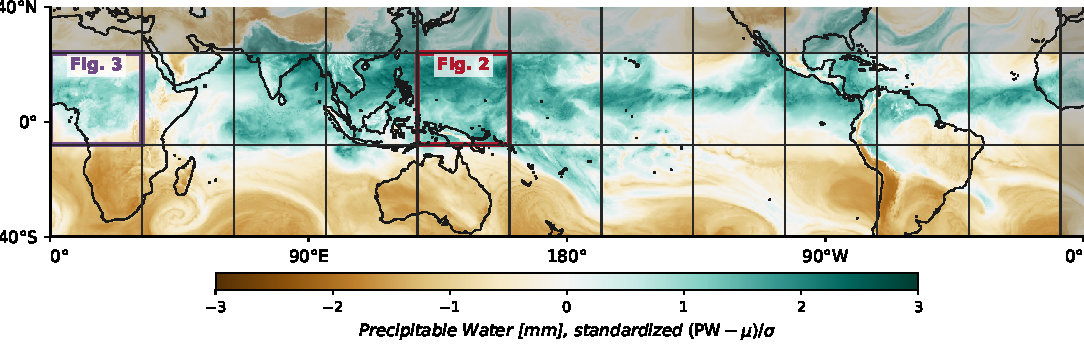
\includegraphics{figures/fig1a_domain.pdf}}
\caption{\textbf{The domain and its tiling.} Precipitable water (mm,
standardized dataset-wide) over the tropical belt ($40^{\circ}$S--$40^{\circ}$N,
$0.25^{\circ}$, one 15-min frame of the 40-day DYAMOND MPAS record), tiled
into the $2 \times 11 = 22$ blocks per day on which all training,
evaluation, and splitting operate; gray strips never enter the pipeline.
The red box marks the example block used in
Figures~\ref{fig:arch} and~\ref{fig:pairs}, over the Maritime Continent /
West Pacific warm pool. Over the 40 days the $880$ (block, day) units are
split $616/132/132$ into train/val/test (Text~S1).}
\label{fig:data}
\end{figure}

\begin{figure}
\centering
\makebox[\textwidth][c]{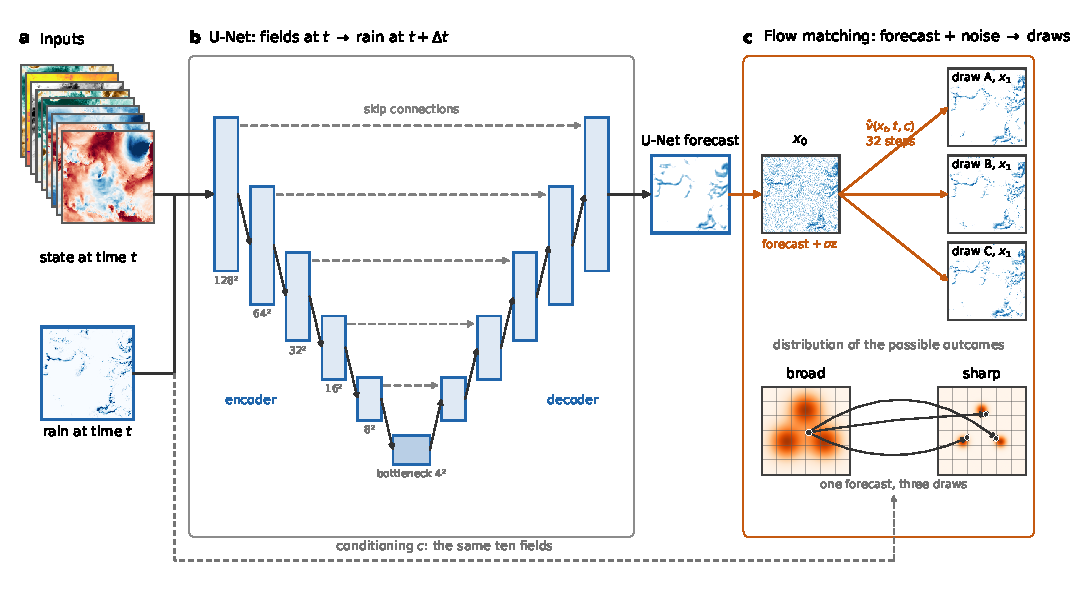
\includegraphics{figures/fig2_pipeline.pdf}}
\caption{\textbf{From the large-scale state to rain draws} (the standard
example block at $+3$~h; all rain maps are model fields on one log color
scale). A.~The inputs at time $t$: nine fields of the large-scale state,
stacked, and the current rain. B.~The U-Net maps these ten fields to the
rain at $t + \Delta t$: an encoder of five stages, a bottleneck, a mirrored
decoder, and skip connections (dashed). Sizes are resolution $\times$ channels. The ten input
fields ($128^2 \times 10$) are reduced to a latent of $4^2 \times 2048$,
the resolution halving and the channels doubling from $64$ at each stage,
and expanded back to two output fields ($128^2 \times 2$): the rain shown
here and a wet/dry field (Figure~S1).
C.~Flow matching. The U-Net forecast plus noise,
$x_0 = z_{\mathrm{fc}} + \sigma\varepsilon$, is the starting state. A
second U-Net of comparable size, the velocity network, returns the velocity $\hat{v}$ at the
current state $x_s$, and the state is advanced by $\hat{v}\,\delta$; this
step is repeated $32$ times and gives one draw $x_1$. Its input has
eleven channels, $x_s$ and the ten input fields (dashed arrow), and its
output one, the
velocity; it also receives the flow time $s$ (not drawn). Three
noise realizations give draws A, B, and C. Bottom: a two-dimensional sketch
of the idea, not of the actual distributions: one uncertain starting point
is carried to definite outcomes, here one draw to one peak and two draws to
another. The ten input maps, the full architecture, and the two outputs of
the U-Net are shown in Figure~S1.}
\label{fig:arch}
\end{figure}

The data are the DYAMOND MPAS-Atmosphere simulation \cite{stevens2019}: a
global storm-resolving run at ${\sim}3.8$~km with output every $15$~min
over a 40-day summer period. Deep convection is resolved by the dynamics
and the cloud microphysics (a double-moment scheme for cloud and rain),
not by a convection scheme. MPAS reproduces the mean precipitation and its
diurnal cycle within the DYAMOND range \cite{stevens2019} but produces more
tropical mesoscale convective systems than IMERG-based tracking finds
\cite{feng2023, feng2025}; the horizons below are therefore horizons of a
simulated atmosphere, measured against the model's own rain. We regrid
the fields to a regular $0.25^{\circ}$ grid (${\approx}28$~km) over
$40^{\circ}$S--$40^{\circ}$N: $320 \times 1440$ pixels, $96$ frames per
day, $40$ days. The rain on this grid is the average of resolved
convection, which keeps the small and short-lived systems that a
parameterization at this resolution does not produce. Nothing below one
pixel is evaluated.

Each frame is tiled into $22$ blocks of $128 \times 128$ pixels
($2 \times 11$; the last $64$ rows and $32$ columns are left out,
Figure~\ref{fig:data}). The unit of the data split is the block-day: one
block location on one day, with all its $96$ frames. The $880$ block-days
are shuffled with a fixed seed and cut into $616$ for training, $132$ for
validation, and $132$ for testing. Blocks do not overlap and a block-day
is never split across sets, so neither a pixel nor the 15-minute
autocorrelation at a fixed location can leak between training and test.
A storm straddling two adjacent blocks in different sets is the residual
risk; the evaluation counts a system in the set of the block that holds
its centroid. An earlier split by day leaked through the autocorrelation
and was discarded; no result here uses it (Text~S1).

Every model takes the same ten input fields at time $t$: precipitable
water, 2-m temperature, outgoing longwave radiation at the top of the
atmosphere, moist static energy and both horizontal wind components at
$850$ and $500$~hPa, and the rain at $t$. Each input is standardized to
zero mean and unit variance with one mean and one standard deviation per
field over the whole record; the rain is transformed to $\ln(1 + R)$
before standardization, $R$ in mm per $15$~min. Giving the model the
current rain means giving it the persistence forecast, so persistence is
nested in every model: any skill above it is skill the model added. The
target is the rain accumulated over $15$~min at $t + \Delta t$, in mm
and not standardized, for $\Delta t = 0.25, 0.5, 1, 2, 3$, and $6$~h.
One model is trained per lead. The models see one $128 \times 128$ block
at a time; nothing outside the block is given to them.

\subsection{Models}\label{sec:unet}

We train two models per lead. The first is deterministic and returns one
rain field; the second is generative, starts from the first's field, and
returns as many different rain fields as one asks for.

\textit{The deterministic U-Net.} It maps the ten input fields to the rain
at $t + \Delta t$ (Figure~\ref{fig:arch}B). It is a U-Net of $125$~M
parameters (Text~S2): five encoder stages, each two $3 \times 3$
convolutions with group normalization and ReLU, from $64$ channels at
$128^2$ pixels to $1024$ at $8^2$; a $2048$-channel bottleneck at $4^2$; a
mirrored decoder with skip connections; and two $1 \times 1$ output
heads. The rain head has a softplus activation, so the rain is
non-negative; the wet/dry head returns logits. The bottleneck is
modulated by the mean and minimum outgoing longwave radiation of the
block through a small network that returns a scale and a shift per
channel (FiLM), which gives the network the convective regime of the block
in one number pair. The loss is
$\mathrm{MSE}_{\mathrm{wet}} + \mathrm{BCE} + 0.25\,\mathrm{FSS}$: the
mean-square error of the rain on the wet pixels of the truth, the binary
cross-entropy of the wet/dry logits against the truth being wet
($R > 0$) on all pixels, and a differentiable fractions skill score at
kernel sizes of $1, 3, 5, 11, 19$, and $33$ pixels ($28$ to $920$~km),
which penalizes rain placed at the wrong scale. Training uses AdamW
(learning rate $10^{-3}$, weight decay $10^{-5}$), batches of $64$
blocks, a learning rate halved every $8$ epochs, and early stopping after
$10$ epochs without improvement of the validation loss ($51$ to $82$
epochs depending on the lead), on one A100 per lead.

A model trained with a mean-square error returns the conditional mean of
the target. For rain this mean is smooth: it spreads each uncertain
system over the area where it might be and lowers its intensity, more so
as the lead grows. The wet/dry head hedges in the same way: because some
rain is present almost everywhere in a $15$-minute kilometer-scale field,
the loss-minimizing answer is to call almost every pixel wet, and it does
(Figure~S1C). Neither head is faulty; both answer the question the loss
asks. The evaluation uses the rain head alone, thresholded, and the
generative model is added to obtain fields that commit to one outcome.

\textit{The generative model, in words.} The U-Net has already placed the
rain; what it cannot do is choose between the outcomes it averages over.
The generative model makes that choice. It takes the U-Net forecast,
adds a little noise to it, and then sharpens the noisy field step by step
into one realistic rain field. Which realistic field comes out depends on
the noise: a different noise gives a different field, and all of them are
consistent with the same smooth forecast and the same inputs. The
sharpening is learned from the training data with flow matching
\cite{lipman2023, liu2023}: a method, not an architecture, that moves a
field continuously from a starting point to an end point in a fictitious
time $s$ from $0$ to $1$ (Figure~\ref{fig:arch}C). The U-Net is trained
first and frozen; the generative model is trained on its forecasts for the
same lead.

\textit{Inputs and outputs.} The generative model works in the log space
$z = \ln(1 + R)/2$. Its input is the U-Net forecast for the block,
$z_{\mathrm{fc}}$, together with the same ten input fields $c$ that the
U-Net saw. Its output is one rain field, a draw, with the shape and units
of the target. Inside, the model is a second U-Net, the velocity network
$\hat{v}(x_s, s, c)$, with the same trunk as the first and a comparable
number of parameters. Its input has eleven channels, the current field
$x_s$ stacked on the ten input fields, plus the time $s$, which scales and
shifts the features at every stage; its output is one field, the velocity,
of either sign: the direction in which each pixel must change at that
moment. It plays the role of the tendency term of a numerical model,
$\mathrm{d}x/\mathrm{d}s$ as a function of the state, learned from data
instead of derived from equations.

\textit{The two end points.} The starting point is the forecast plus
noise,
\begin{equation}
x_0 = z_{\mathrm{fc}} + \sigma\,\varepsilon, \qquad
\varepsilon \sim \mathcal{N}(0, I),
\end{equation}
with $\varepsilon$ a field of independent Gaussian numbers. The amplitude
$\sigma$ is not tuned: it is the root-mean-square error of the U-Net
forecast on the wet pixels of the training set, in $z$, at that lead
($0.10, 0.12, 0.15, 0.17, 0.19$, and $0.20$ for the six leads). The end
point $x_1$ is the true field at the same valid time.

\textit{Training.} For each example we draw $\varepsilon$ and a time $s$
uniform in $[0, 1]$, and form the point on the straight line between the
end points,
\begin{equation}
x_s = (1 - s)\,x_0 + s\,x_1 .
\end{equation}
Along this line the velocity is constant, $x_1 - x_0$, and the network is
trained to return it:
\begin{equation}
\mathcal{L} = \big\langle\, \| \hat{v}(x_s, s, c) - (x_1 - x_0) \|^2
\,\big\rangle .
\end{equation}
Each forecast is paired with its own truth, so the lines are short: the
network learns a correction to the forecast, not a rain field from pure
noise. Optimizer, batches, and stopping rule are those of the U-Net.

\textit{Sampling.} To produce one draw we draw $\varepsilon$, form $x_0$,
and integrate $\mathrm{d}x/\mathrm{d}s = \hat{v}(x_s, s, c)$ from $s = 0$
to $1$ with $32$ steps of Heun's method, the second-order
predictor--corrector: a trial Euler step with the velocity at the current
state, then the update with the mean of the velocities at the current and
trial states. The network is evaluated at $s = 0, 1/32, \ldots, 31/32$,
twice per step except the last, which is a plain Euler step: $63$
evaluations per draw. The field at $s = 1$, transformed back to mm, is the
draw. Nothing is learned at this stage.

\textit{Noise and scoring.} The noise is the only source of randomness;
with $\sigma = 0$ the flow is a deterministic correction. Each
$\varepsilon$ gives a different sharp field consistent with the same
smooth forecast (Figure~\ref{fig:arch}C). All statistics of the flow in
this paper are computed on one draw per block and frame, with a fixed
seed, and never on an average of draws: the average of draws is again an
estimate of the mean and would remove the difference we measure. A
denoising diffusion model started from the same forecast was also tested;
its small-scale variance saturates at $0.80$--$0.85$ of the truth's,
because it is trained to denoise noised truth and applied to noised
forecasts, and it is reported as a sensitivity in Text~S3.

\subsection{Evaluation: systems, matching, and the horizon}
\label{sec:evaluation}

\textit{Systems.} In the truth and in each forecast, a system is an
8-connected set of pixels with rain above $0.1$~mm per $15$~min. Pixel
areas follow the cosine of latitude. A system has an area $A$ (km$^2$), a
total rain $P$ (mm\,km$^2$), a mean intensity $\rho = P/A$, so that
$P = \rho A$ exactly, and a size $L = \sqrt{A}$. One pixel is $L \approx
28$~km; the smallest systems evaluated are one pixel.

\textit{Matching.} Within each frame, the intersection over union (IoU) is
computed between every truth system and every forecast system. Pairs are
accepted in decreasing order of IoU, each system at most once, down to
$\mathrm{IoU} = 0.1$. Every system then has one of three roles: matched,
missed (a truth system without partner), or false alarm (a forecast system
without partner). In each size band, the probability of detection is
$\mathrm{POD} = \mathrm{matched}/(\mathrm{matched} + \mathrm{missed})$,
counted on truth systems, and the false-alarm ratio is $\mathrm{FAR} =
\mathrm{false\ alarms}/(\mathrm{matched} + \mathrm{false\ alarms})$,
counted on forecast systems. The bands are ten, log-spaced, from $25$ to
$600$~km for the curves at one lead (Figure~\ref{fig:horizon}A,B) and
from $25$ to $800$~km for the horizon (Figure~\ref{fig:horizon}C,D).

\textit{Area and intensity errors.} For a matched pair,
$\mathrm{d}\ln A = \ln(A_{\mathrm{fc}}/A_{\mathrm{truth}})$ and
$\mathrm{d}\ln\rho = \ln(\rho_{\mathrm{fc}}/\rho_{\mathrm{truth}})$, so
that $\mathrm{d}\ln P = \mathrm{d}\ln A + \mathrm{d}\ln\rho$; negative
means too small or too weak, and a given relative error weighs the same
on a $30$-km cell and a $400$-km system. Band means are weighted by the
truth system's rain $P$, in three bands: below $65$~km, $65$ to $200$~km,
above $200$~km.

\textit{Horizon.} In each size band, $\mathrm{POD}(t)$ is taken at the six
leads and divided by its value at the shortest lead, $15$~min. The horizon
$\tau(L)$ is the e-folding time of a least-squares fit of
$\exp[-(t - 0.25\,\mathrm{h})/\tau]$ to that ratio, with $\tau$ bounded to
$[0.1, 200]$~h. The power law $T(L) \propto L^{\alpha}$ is fitted by
unweighted least squares in $\ln\tau$ against $\ln L$ on the six bands
from $59$ to $336$~km, the same for all forecasts. The two smallest bands
are left out because their systems are one to two pixels wide, and the
two largest because their $\tau$ exceeds the $6$~h covered by the leads
several times over and is an extrapolation.

\textit{The null.} Persistence, the rain at $t$ taken as the forecast for
$t + \Delta t$, goes through the same detection, matching, bands, and
fits. It is a strong null for detection at this matching: a long-lived
system still overlaps its own earlier position at $\mathrm{IoU} \ge 0.1$.
The sensitivity of every result to the IoU threshold, the rain threshold
and one-to-one matching is reported in Text~S4.

%% ===================== 3. RESULTS ==========================================
\section{Results}\label{sec:results}

\subsection{A realistic forecast: from the conditional mean to flow draws}
\label{sec:res-model}

The two-head forecast has the right pattern and the wrong texture. On the
example block at $+3$~h (Figures~\ref{fig:arch} and~\ref{fig:pairs}) it places rain where
the truth has rain, but as a smooth envelope: it draws $22$ systems where
the truth holds $120$, and its peaks are under-drawn. This is the
conditional mean at work, and it ages: the forecast's wet-masked error in
log-rain space, the $\sigma$ handed to the flow, doubles from $0.10$ at
$+15$~min to $0.20$ at $+6$~h, and the field loses contrast as the
distribution it averages over widens.

The flow draws do not age that way. Started from the same forecast plus
noise of amplitude $\sigma$, each draw is a sharp field with the cells and
the intensities of the truth, at every lead. Two draws agree where the
forecast is certain and differ where it is not
(Figure~\ref{fig:arch}C, draws A to C): the uncertainty that the
U-Net stamps into the field as blur appears in the flow as displaced
systems. A sharp field can be sharply wrong, so realism is not yet skill.
Whether it is skill, and at which scales, is the next question.

\subsection{Skill across scales: the rain decomposition}
\label{sec:res-scales}

\begin{figure}
\centering
\makebox[\textwidth][c]{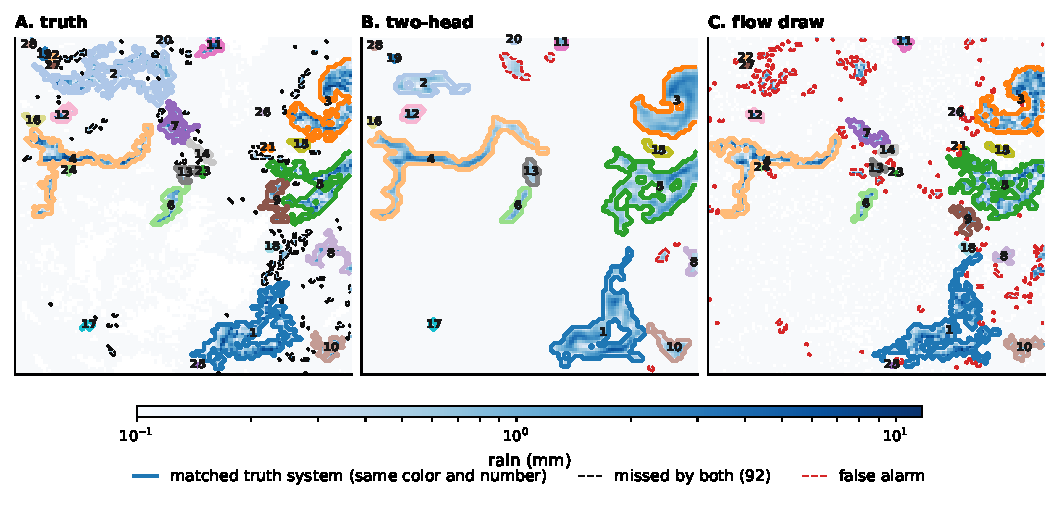
\includegraphics{figures/fig3_pairs.pdf}}
\caption{\textbf{The instrument on one frame} ($+3$~h, the standard example
block over the Maritime Continent; the truth on the left, the two forecasts
on the right). Top: the rain fields of the truth (A), the two-head U-Net
(B), and one flow draw (C), on one log color scale, with the matched pairs
outlined and numbered: one color and number per truth system, the same in
every panel where a model found it. Bottom: the outcome of the matching (systems $>0.1$~mm,
8-connected; greedy one-to-one, $\mathrm{IoU} \ge 0.1$). D.~The $120$ truth
systems: green if found by both models ($11$), blue if missed by the U-Net
only ($11$), purple if missed by the flow only ($6$), black if missed by
both ($92$, overwhelmingly the smallest). E.--F.~For each forecast, its matched
systems (green) and its false alarms (forecast systems matching nothing,
red). The flow finds $22$ systems where the U-Net finds $17$, and produces
many more small false alarms, $106$ against $5$.}
\label{fig:pairs}
\end{figure}

\begin{figure}
\centering
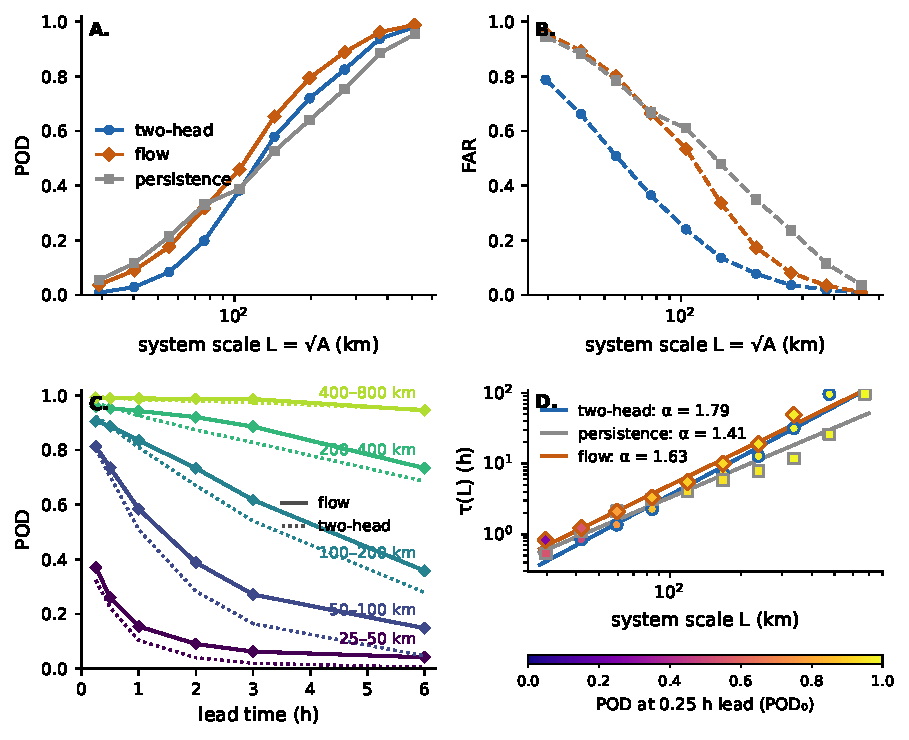
\includegraphics[width=\textwidth]{figures/fig5_horizon.pdf}
\caption{\textbf{Skill by scale and the predictability horizon} (full held-out
record: $132$ test blocks $\times$ $40$ days, ${\sim}10^6$ systems per model
and lead). A.~Probability of detection and B.~false-alarm ratio by system
scale $L$ at $+3$~h for the two-head model, persistence, and the flow (per
draw). C.~POD decay with lead time per scale band (solid: flow; dotted:
two-head). D.~The e-folding time $\tau(L)$ fitted across the six trained
leads, with power-law fits $T(L) \propto L^{\alpha}$ on the six bands from
$59$ to $336$~km (shaded), the same for the three forecasts:
$\alpha = 0.97$ (persistence), $1.77$ (two-head), $1.78$ (flow). Filled
markers enter the fit and are colored by each band's $\mathrm{POD}_0$;
hollow markers are left out. Above the dotted line $\tau$ exceeds the
longest trained lead and is an extrapolation of the exponential fit.}
\label{fig:horizon}
\end{figure}

Figure~\ref{fig:pairs} shows the instrument at work on one frame: of $120$
truth systems the two-head matches $17$ and the flow draw $22$, at the price
of $106$ false alarms against $5$, and the $92$ systems found by neither are
overwhelmingly the smallest. The statistics that follow
pool ${\sim}10^6$ such systems per model and lead over the full held-out
record ($132$ test blocks $\times$ $40$ days).

Detection is a function of size before it is a function of the model
(Figure~\ref{fig:horizon}A). At $+3$~h the flow's POD rises from $0.04$ at
$L \approx 30$~km to $0.98$ at $480$~km, and the two-head and persistence
climb the same ramp. The flow sits above the two-head in every scale band
($0.79$ vs $0.72$ at $L \approx 190$~km), and below $65$~km its POD nearly
triples ($0.078$ vs $0.028$). The instrument prices the gain in the same
breath (Figure~\ref{fig:horizon}B): below $65$~km the flow's FAR is $0.92$
against $0.64$ --- it finds small storms by proposing many --- while at
$190$~km it is $0.17$ against the two-head's $0.08$ and persistence's
$0.35$. Persistence remains a strong null at this lead: its POD is $0.64$
at $190$~km and, below ${\sim}70$~km, above the flow's ($0.25$ vs $0.22$
at $60$~km), because a long-lived storm still overlaps its own
past at $\mathrm{IoU} \ge 0.1$ (Text~S4).

\begin{figure}
\centering
\makebox[\textwidth][c]{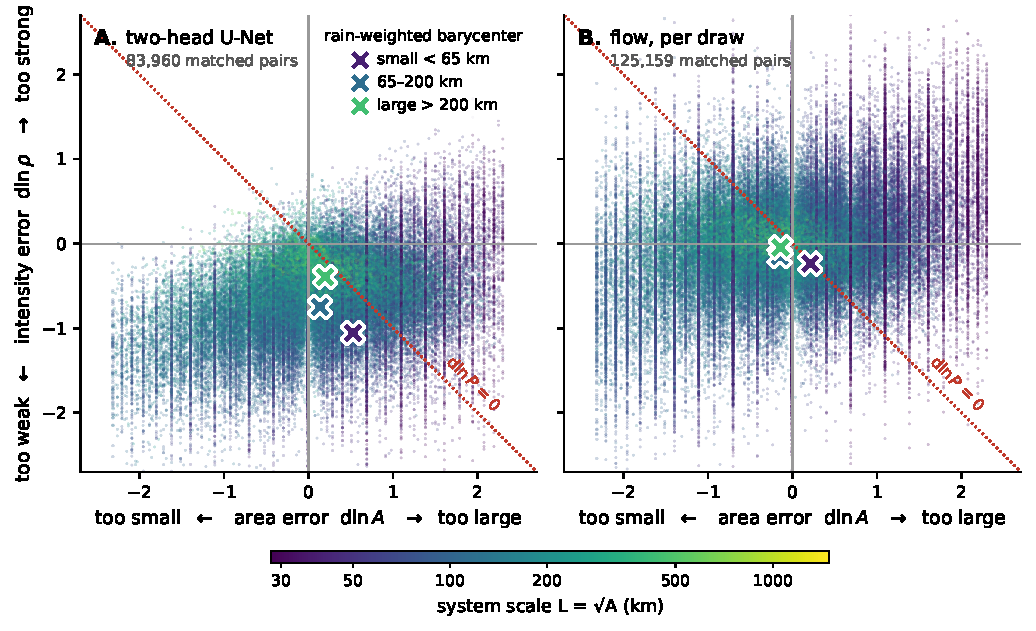
\includegraphics{figures/fig4_decomp.pdf}}
\caption{\textbf{Area and intensity errors of the matched systems}
($+3$~h, full held-out record; identical axes in the two panels). Each
matched truth--forecast pair has an area error $\mathrm{d}\ln A$ and an
intensity error $\mathrm{d}\ln\rho$. The grey outline encloses $95\%$ of all
matched pairs. For each of three size bands, small ($<65$~km), medium
($65$--$200$~km), and large ($>200$~km), the shaded region holds $75\%$ of
the band's pairs, darker where the pairs are denser; both regions are
highest-density regions of a smoothed two-dimensional histogram. The dot
is the precipitation-weighted mean error of the band, joined to the origin.
Along the dotted diagonal, $\mathrm{d}\ln P = 0$, area and intensity errors
cancel exactly.
A.~The two-head U-Net ($83{,}960$ pairs): systems are too large and too
weak, most of all the small ones, $(+0.53, -1.05)$.
B.~The flow, per draw ($125{,}159$ pairs): the mean errors move toward the
origin at every scale (small $(+0.21, -0.24)$, medium $(-0.15, -0.15)$,
large $(-0.14, -0.04)$).}
\label{fig:decomp}
\end{figure}

Matched pairs say what the detected systems look like
(Figure~\ref{fig:decomp}). At $+3$~h the pairs of the two-head model sit in
a quadrant of compensating errors: band barycenters
$(\mathrm{d}\ln A, \mathrm{d}\ln\rho) = (+0.53, -1.05)$ for small systems,
$(+0.14, -0.75)$ at mid scales, $(+0.20, -0.39)$ for large --- systems too
large and too weak, with the two errors partially canceling in
$\mathrm{d}\ln P$, which is why aggregate scores miss them. This is the
signature of the conditional mean, and it grows toward small scales.

The flow removes the pathology it was trained on. On identical axes
(Figure~\ref{fig:decomp}B) the band barycenters collapse toward the origin:
small systems to $(+0.21, -0.24)$, mid to $(-0.15, -0.15)$, large to
$(-0.14, -0.04)$. Size and intensity are restored at every scale, per draw
--- these are single sharp realizations, not an ensemble mean.

\subsection{The time horizon of each scale}\label{sec:res-horizon}

Detection decays with lead in every size band, faster for small systems
(Figure~\ref{fig:horizon}C), and the decay is close to exponential; its
e-folding time is the horizon of the band. Fitted across the six leads
(Figure~\ref{fig:horizon}D), the horizon of the flow rises from
$\tau = 0.83$~h for the smallest resolved systems ($L \approx 30$~km) to
$10$~h at $170$~km and beyond a day above $400$~km, and follows a power law
$T(L) \propto L^{\alpha}$ with $\alpha = 1.63$. The two-head gives
$\alpha = 1.79$ and persistence $\alpha = 1.41$.

The null orders the three forecasts. The two-head and persistence curves
cross near $L \approx 100$~km: above it the model separates cleanly from
the null, below it persistence wins ($\tau = 0.84$~h vs $1.10$~h at
$42$~km) --- small, short-lived convection is where the deterministic
forecast has nothing to add over the observation that storms briefly
persist. The flow removes the crossover. Its $\tau(L)$ is above the
two-head's in every band the six leads constrain and at or above
persistence's in every band
($0.83$~h vs $0.55$ and $0.53$~h at $30$~km; the two are tied at $60$~km,
$2.09$ vs $2.11$~h), making it the first forecast in this study that the
nested null does not beat at any scale.

Because the flow's gain is largest at small scales, the measured exponent
\emph{flattens}, from $1.79$ to $1.63$: $\alpha$ measures how horizon is
shared between large and small systems, not how much of it there is, and
the deterministic model's excess slope was the blur taxing small systems
--- estimator artifact, not atmosphere.

\subsection{The same lens on operational AI forecasts}\label{sec:res-wb2}

\begin{figure}
\centering
\makebox[\textwidth][c]{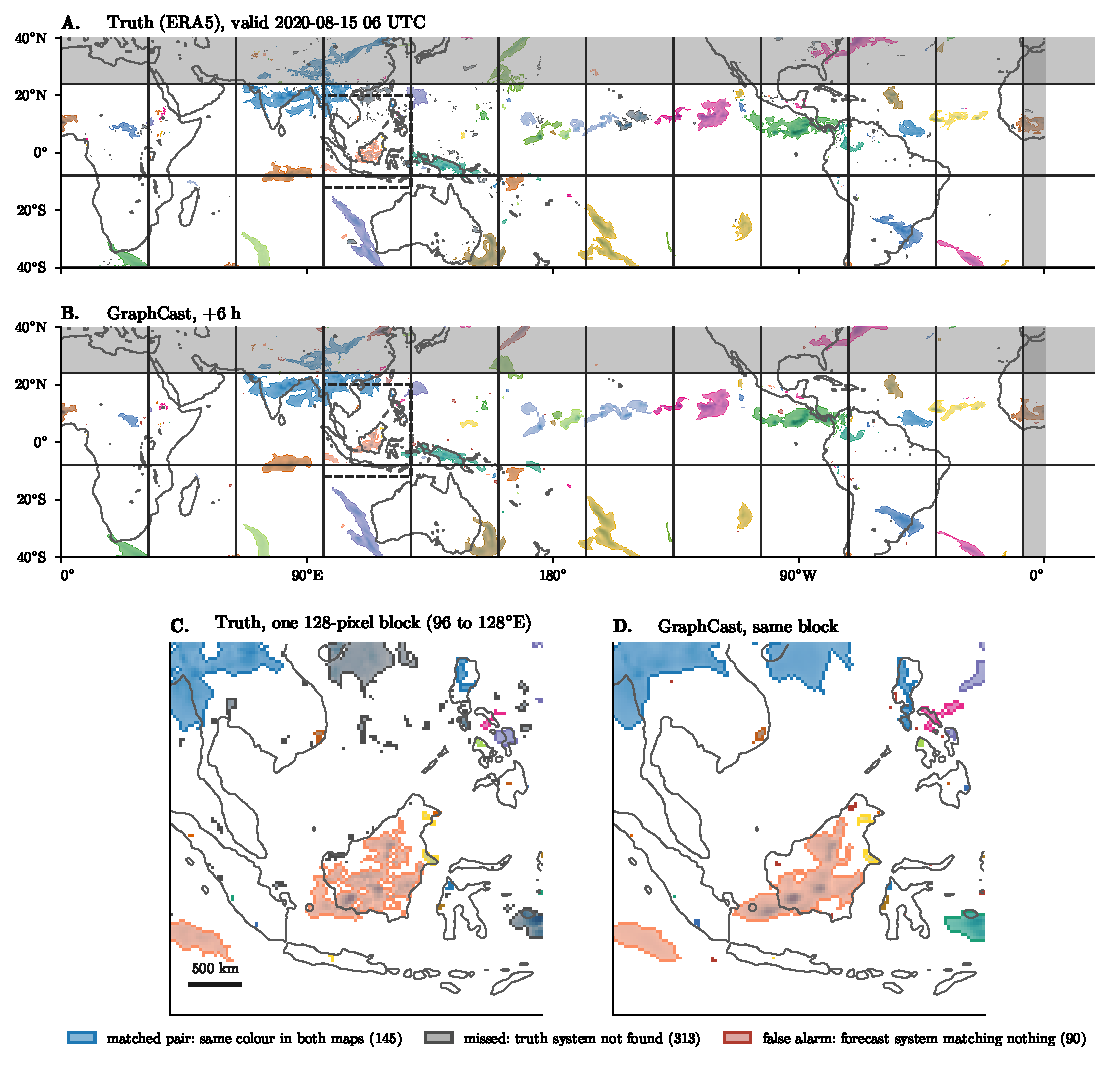
\includegraphics{figures/fig7a_wb2maps.pdf}}
\caption{\textbf{Pair recognition on an operational forecast} (GraphCast
$+6$~h, ERA5 truth, valid 2020-08-15 06 UTC; threshold $2.4$~mm/6~h --- the
rate equivalent of the km-scale $0.1$~mm/15~min; $\mathrm{IoU} \ge 0.1$).
A.--B.~The full tropical belt on the block grid of Figure~\ref{fig:data}:
matched pairs share a color across the two maps ($145$); the dashed box
marks the zoom block. C.--D.~The $128$-pixel zoom (the LatentSky patch size; Maritime
Continent, $96$--$128^{\circ}$E): the large systems are found, the small ones are not. The zoom alone shows,
in black, the missed truth systems in C and GraphCast's false alarms in D
($313$ and $90$ over the whole belt).}
\label{fig:wb2maps}
\end{figure}

\begin{figure}
\centering
\makebox[\textwidth][c]{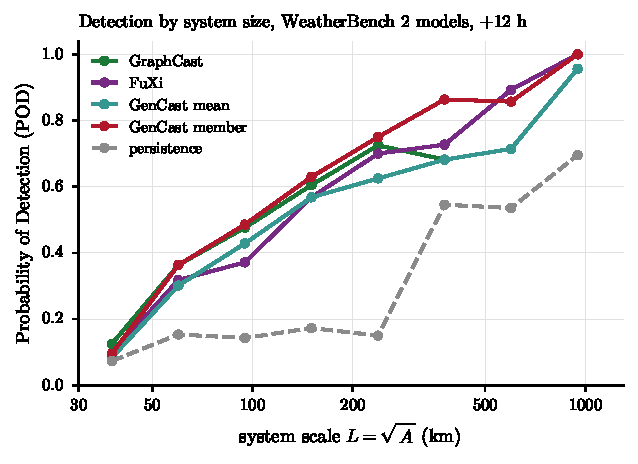
\includegraphics{figures/fig7b_pod.pdf}}
\caption{\textbf{Detection and false alarms by scale for the WB2 models} at
$+12$~h (2020-08-15, two initializations; same threshold and matching as
Figure~\ref{fig:wb2maps}). A.~Probability of detection and B.~false-alarm
ratio by system size. A single GenCast member is the best forecast from
${\approx}240$~km up ($0.78$--$0.82$) at a FAR cost ($0.32$ vs GraphCast's
$0.17$); the ensemble mean falls back into the deterministic pack; below
$60$~km every model is at $\mathrm{POD} \le 0.13$. Bands with fewer than
$20$ systems are left blank.}
\label{fig:wb2pod}
\end{figure}

\begin{figure}
\centering
\makebox[\textwidth][c]{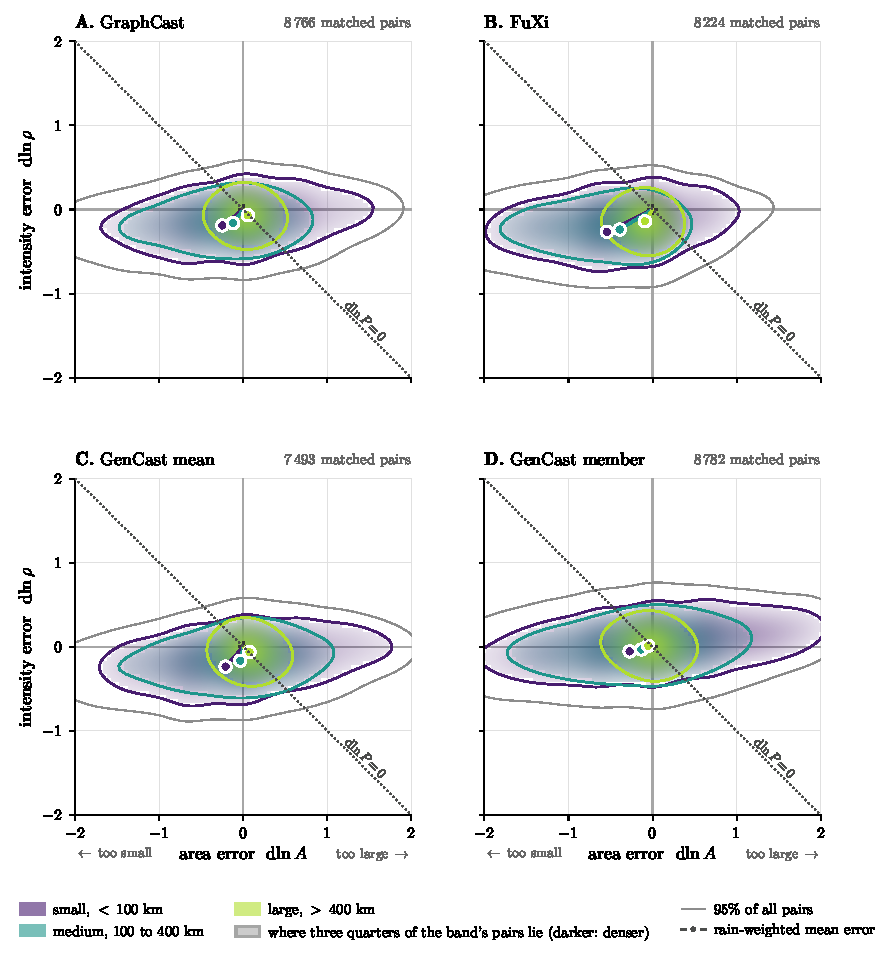
\includegraphics{figures/fig7c_clouds.pdf}}
\caption{\textbf{The error decomposition on the WB2 models} ($+12$~h, August
2020 month-pooled, ${\sim}8{,}000$ matched pairs per model; conventions as
in Figure~\ref{fig:decomp}, with the size bands $<100$~km, $100$--$400$~km,
and $>400$~km). The deterministic too-weak bias (mean $\mathrm{d}\ln\rho$
of $-0.24/-0.17/-0.06$ from small to large) is erased by the diffusion
member ($-0.06/-0.03/+0.01$). The clouds are wide in $\mathrm{d}\ln A$ and
narrow in $\mathrm{d}\ln\rho$ --- the reverse of the km-scale clouds: at
$0.25^{\circ}$ the rate is recoverable, the boundaries are not.}
\label{fig:wb2clouds}
\end{figure}

The evaluation transfers unchanged to WeatherBench~2
(Figures~\ref{fig:wb2maps}--\ref{fig:wb2clouds}): GraphCast, FuXi, GenCast,
and FGN against ERA5 over the same tropical belt, at rate-equivalent thresholds
($2.4$~mm per $6$~h $=$ the km-scale $0.1$~mm per $15$~min). This part is an
outlook, not a ranking against LatentSky --- different data, resolution, and
leads. Three observations carry it.

First, the identical scale story: POD rises monotonically with $L$ for every
model, and below $L \approx 60$~km every model --- deterministic or generative
--- sits at $\mathrm{POD} \le 0.13$ at $+6$ and $+12$~h, already a medium lead
for convection. Second, sampling helps where the models are competent:
at $+12$~h a single GenCast member gives the highest POD of any forecast from
${\approx}240$~km up ($0.78$--$0.82$ vs GraphCast's $0.68$--$0.73$), at a FAR
cost ($0.32$ vs $0.17$), while the GenCast ensemble mean falls back into the
deterministic pack --- the per-draw scoring rule matters as much for
operational models as for ours. Third, over a full month of matched systems
(${\sim}8{,}000$ pairs per model), the deterministic models carry a systematic
too-weak bias worst at small scales ($\mathrm{d}\ln\rho$ barycenters $-0.24$,
$-0.17$, $-0.06$ from small to large bands), and the diffusion member erases it
at every scale ($-0.06$, $-0.03$, $+0.01$). The error clouds are wide in
$\mathrm{d}\ln A$ and narrow in $\mathrm{d}\ln\rho$ --- the reverse of the
km-scale clouds: at $0.25^{\circ}$ the rain rate is recoverable but the system
boundaries are not.

The small-system floor itself, however, is not an indictment of resolution
alone --- our own scaling law prices the lead. With
$\tau(30~\mathrm{km}) \approx 0.8$~h even for the flow at kilometer scale, a
$+6$~h forecast asks for detection seven e-folding times past the horizon: no
model, at any resolution, should find a $30$-km system at $+6$ or $+12$~h.
The two arguments therefore compose rather than compete. Kilometer-scale data
is necessary for small systems to be \emph{representable} at all, and
sub-hour forecast cadence is necessary to catch them \emph{within their
horizon}; operational systems stepping at $6$~h fail both conditions at once,
and fixing the resolution without the cadence would move nothing below
${\sim}60$~km.

%% ===================== 5. DISCUSSION =======================================
\section{Discussion and outlook}\label{sec:discussion}
%% DRAFT for Sophie's rewrite — ~750 words, room left for additions

What does the horizon measure, and what does it not? Systems are matched at
a common valid time, so $T(L)$ does not follow individual storms through
their life cycles; it asks the operational question --- is the rain where the
forecast said it would be, when it said it would be there? Time evolution
enters statistically, through the family of six leads: the decay of
detection with lead time is precisely the rate at which the evolving
atmosphere carries systems away from any snapshot-consistent prediction, and
the persistence null makes this reading exact, because persistence is the
forecast with \emph{no} evolution at all. The margin over persistence is
therefore the evolution the model captured. A Lagrangian companion ---
tracking matched systems through consecutive frames to separate displacement
error from genuine dissipation and initiation --- is the natural next
instrument, and the matched-pair tables built here already contain the
centroids it needs.

The trigger--amplitude decomposition can be made quantitative. Writing the
total error schematically as
$\epsilon(t) = \epsilon_{\mathcal{T}}(t) + \epsilon_A(t)$, the decay of
detection measures the trigger term and the matched-pair intensity error
measures the amplitude term, conditional on the trigger being found. Two
predictions follow from the physical picture. First,
$\epsilon_{\mathcal{T}}$ should grow faster with lead than $\epsilon_A$ ---
the environment that controls amplitude carries the longer memory --- and
our curves are consistent with this ordering: detection collapses within
$\tau(L)$ while the matched $\mathrm{d}\ln\rho$ barycenters drift only
slowly with lead. Second, and testable with the input ablations this
framework invites, the decay timescale $\tau$ should be a property of the
atmosphere rather than of the input set: enriching the inputs (thermodynamic
profiles, explicit vertical motion) should raise the intercept
$\mathrm{POD}_0$ but leave $\tau$, and hence $\alpha$, unchanged. If instead
$\tau$ moves, the horizon is partly informational, not intrinsic --- either
outcome is instructive.

The exponent itself deserves a careful reading, because the natural
intuition --- a better model should have a larger $\alpha$ --- is wrong.
$\alpha = \mathrm{d}\ln\tau / \mathrm{d}\ln L$ measures how horizon is
\emph{distributed} between large and small systems; skill lives in the level
of $\tau(L)$, which the flow raises at every scale. The measured values then
order themselves physically. Detection dies when the position error of a
system becomes comparable to its own size, so if that error grows as
$t^{p}$, then $\alpha = 1/p$. Persistence ($\alpha = 1.41$,
$p \approx 0.7$) is close to pure advection: the storm is simply carried away. The
trained models know the steering flow, remove the coherent part of the
displacement error, and leave a residual wander between advective and
diffusive ($\alpha = 1.63$, $p \approx 0.6$; pure diffusion would give
$\alpha = 2$). The deterministic model's steeper $1.79$ is this intrinsic
slope plus a blur tax that falls hardest on small systems; the flow removes
the tax and recovers ${\approx}1.6$, our best estimate of the intrinsic
exponent. Lorenz's dry-cascade value, $\tau \propto \ell^{2/3}$
\cite{lorenz1969}, sits far below all of these --- detection of intermittent
precipitation objects dies by displacement against size, not by
inertial-range error saturation. The reading is falsifiable with the tables
already in hand: the centroid separations of matched pairs should grow as
$t^{1/\alpha}$ with each forecast's own exponent, and the flow's extra
small-system matches should come through size and shape, not through better
centroids.

Several limitations bound the claims. The record is one 40-day tropical
summer of a single kilometer-scale model, and MPAS overestimates deep
convection relative to observations; the exponents deserve re-measurement on
other DYAMOND members and on observations (IMERG at its native scales) before
they are treated as universal. The two largest scale bands barely decay
within the trained $6$~h, so their $\tau$ is an extrapolation of the fit,
not a measurement. The matching itself has known sensitivities --- loose IoU
flatters persistence, the rain threshold changes the object population ---
quantified in Text~S4; none changes the ordering of the three forecasts. And
our generative claims are per-draw statements about single realizations;
building and scoring proper ensembles from the flow (spread, calibration,
CRPS) is a separate study.

The practical implication is a recipe rather than a model. The apparent
predictability limit of km-scale precipitation contains a large,
recoverable estimator artifact, and the recovery mechanism is cheap: a
generative correction trained on the forecast's own error budget, sampled
per draw, with the false-alarm price stated by the same instrument that
measures the gain. The WB2 results suggest the recipe transfers: GenCast's
members --- but not their mean --- already behave like the flow, which
argues that joint sampling of the precipitation field, rather than
per-pixel-optimal objectives, is the property to preserve as operational
models evolve. For the smallest systems the recipe alone is not enough:
their horizon is shorter than any operational forecast step, so progress
below ${\sim}60$~km requires kilometer-scale training data \emph{and}
sub-hour forecast cadence together. Where the horizon itself varies --- land
versus ocean, tropics versus midlatitudes --- is open, and the instrument
travels: any forecast that produces a rain field, numerical or neural,
deterministic or generative, can be placed on the same $\tau(L)$ axes.

\section{Open Research}
The DYAMOND MPAS output is available through the DYAMOND initiative
\cite{stevens2019}; the regridded $0.25^{\circ}$ tropical-belt fields, the
trained model checkpoints, and the full matched-system tables that underlie
every figure will be archived with a DOI upon acceptance
%% TODO: mint the archive (Zenodo or NCAR GDEX) before submission
. The WeatherBench~2 forecasts (GraphCast, FuXi, GenCast, FGN) and the ERA5
verification fields are publicly available from the WeatherBench~2 cloud
archive \cite{rasp2024}. All analysis and figure code --- the object
detection, matching, and $\rho A$ decomposition, the training and sampling
code for both models, and one script per figure --- is available at
%% TODO: public repository URL
the project repository.

\acknowledgments
Computing resources were provided by the NSF National Center for
Atmospheric Research (CISL), on the Casper and Derecho systems under
allocation UCLB0066. We thank the DYAMOND initiative and the MPAS group at
NCAR for the storm-resolving simulation, the WeatherBench~2 team for the
open forecast archive, and ECMWF for ERA5.

\bibliography{refs}

\end{document}
